\chapter{Apartado B: \textbf{Detección de líneas rectas}}
\label{chapter:tarea_b}

\section*{Tarea B.1: Aplicación de Canny}
\phantomsection
\addcontentsline{toc}{section}{Tarea B.1: Aplicación de Canny}

Para obtener los bordes de las imágenes, aplique el método \texttt{cv2.Canny()} \footnote{ \href{https://docs.opencv.org/3.4/dd/d1a/group\_\_imgproc\_\_feature.html\#ga04723e007ed888ddf11d9ba04e2232de}{Documentación del método \texttt{cv2.Canny()} en OpenCV:} \\{https://docs.opencv.org/3.4/dd/d1a/group\_\_imgproc\_\_feature.html\#ga04723e007ed888ddf11d9ba04e2232de}} de OpenCV a las imágenes de trabajo ajustando los hiperparámetros.

Recuerde que para aplicar Canny, primero deberá pasar su imagen a escala de grises con el método \texttt{cvtColor()}. Por otro lado, observe que el método Canny devuelve una imagen binaria (blanco y negro) con los bordes detectados.


\section*{Tarea B.2: Visualización de líneas}
\phantomsection
\addcontentsline{toc}{section}{Tarea B.2: Visualización de líneas}

Implemente la función \texttt{draw\_lines()} para pintar las líneas detectadas sobre las imágenes. Para ello, puede utilizar el método \texttt{cv2.line()} \footnote{ \href{https://docs.opencv.org/3.4/d6/d6e/group\_\_imgproc\_\_draw.html\#ga7078a9fae8c7e7d13d24dac2520ae4a2}{Documentación del método \texttt{cv2.line()} en OpenCV:} \\{https://docs.opencv.org/3.4/d6/d6e/group\_\_imgproc\_\_draw.html\#ga7078a9fae8c7e7d13d24dac2520ae4a2}} de OpenCV.


\section*{Tarea B.3: Aplicación de transformada de Hough}
\phantomsection
\addcontentsline{toc}{section}{Tarea B.3: Aplicación de transformada de Hough} 
Aplique el método \texttt{cv2.HoughLinesP()} \footnote{ \href{https://docs.opencv.org/3.4/dd/d1a/group\_\_imgproc\_\_feature.html\#ga8618180a5948286384e3b7ca02f6feeb}{Documentación del método \texttt{cv2.HoughLinesP()} en OpenCV:} \\{https://docs.opencv.org/3.4/dd/d1a/group\_\_imgproc\_\_feature.html\#ga8618180a5948286384e3b7ca02f6feeb}} de OpenCV a las imágenes de trabajo y afine los hiperparámetros para extraer las líneas de interés. La Figura \ref{fig:ejemplo_hough} muestra el resultado esperado al aplicar la transformada de Hough sobre una de las imágenes.

\begin{figure}[H]
    \centering
    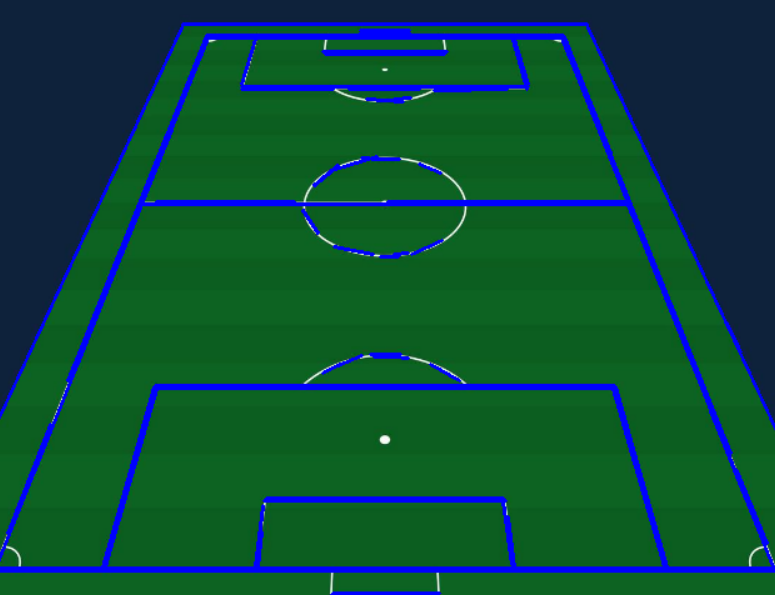
\includegraphics[width=0.3\textwidth]{Lab_3/template/figures/football_lines.png}
    \caption{Ejemplo de detección de líneas con el método Hough.}
    \label{fig:ejemplo_hough}
\end{figure}


\section*{Preguntas}
\addcontentsline{toc}{section}{Preguntas}

\vspace{5mm}
\begin{tcolorbox}[colback=gray!10, colframe=gray!30, coltitle=black, title=Pregunta B.1, halign=left]
Repita el procedimiento para extraer las líneas de las dos imágenes restantes.
\end{tcolorbox}